% !TEX root = B&G_oefeningen.tex
\chapter{Binaire Heap - verdieping}


\begin{oef}
\papier Stel dat we een binaire max-heap hebben geconstrueerd met de code uit dat hoofdstuk.
Welke van de volgende lijst van getallen is mogelijk?
\begin{oefenumerate}
\item $[25, 12, 16, 13, 10, 8, 14]$
\item $[25, 14, 16, 13, 10, 8, 12]$
\item $[25, 14, 12, 13, 10, 8, 16]$
\end{oefenumerate}
\begin{opl}
Het volstaat om de getallen in een boom te zetten en te kijken of de max-heap eigenschap gerespecteerd is. Het juiste antwoord is b), maar wel zullen bij wijze van uitleg laten zien waarom antwoord a) niet correct is. Zet de zeven getallen in volgorde in een complete binaire boom. Je bekomt figuur~\ref{fig:foutemaxheap}. Voor een max-heap moet elke ouder groter zijn dan zijn eventuele kinderen. Aan deze eis is niet voldaan door de knopen met de getallen 12 en 13.
\begin{figure}[htbp]
    \centering
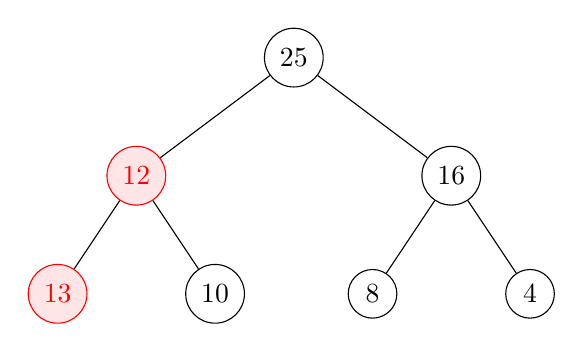
\begin{tikzpicture}[every node/.style={circle,draw},
				level 1/.style={sibling distance=40mm},
				level 2/.style={sibling distance=20mm}]
\node {25}
child { node[red, fill=red!10] {12} 
	child { node[red, fill=red!10] {13} }
	child { node {10}}
}
child { node {16}
	child { node {8}}
	child { node {4}}
};
\end{tikzpicture}
\caption{Foute max-heap uit a)}
    \label{fig:foutemaxheap}
\end{figure}
\end{opl}

\end{oef}



\begin{oef}
\papier De getallen 32, 15, 20, 30, 12, 25 en 16 worden \emph{in die volgorde} toegevoegd aan een binaire max-heap. Welke van volgende getallenlijst is de juiste volgorde in de arraylist?
\begin{oefenumerate}
\item $[32, 30, 25, 15, 12, 20, 16]$
\item $[32, 25, 30, 12, 15, 20, 16]$
\item $[32, 30, 25, 15, 12, 16, 20]$
\item $[32, 25, 30, 12, 15, 16, 20]$
\end{oefenumerate}

\begin{opl}
Voeg alle elementen element per element toe, gevolgd door een eventuele “bubble up”. Je bekomt figuur~\ref{fig:maxheapbubbleup} en dus antwoord a).
\begin{figure}[htbp]
    \centering
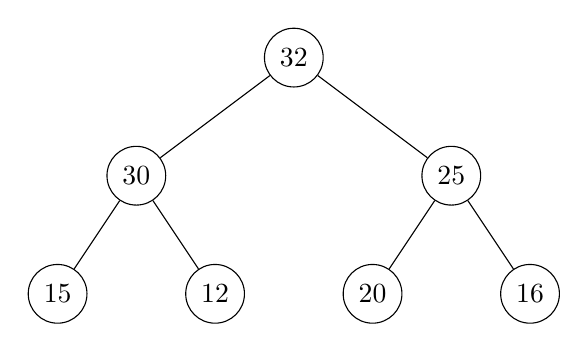
\begin{tikzpicture}[every node/.style={circle,draw},
				level 1/.style={sibling distance=40mm},
				level 2/.style={sibling distance=20mm}]
\node {32}
child { node {30} 
	child { node {15} }
	child { node {12}}
}
child { node {25}
	child { node {20}}
	child { node {16}}
};
\end{tikzpicture}
\caption{Max-heap met de getallen 32, 15, 20, 30, 12, 25 en 16 in die volgorde toegevoegd}
    \label{fig:maxheapbubbleup}
\end{figure}
\end{opl}

\end{oef}


\begin{oef}
\papier \emph{(Examen augustus 2019)} Een binaire min-heap wordt gemaakt door elk getal in het interval $[1, 1023]$ juist één keer te gebruiken. Wat is de maximale diepte waarop het getal 9 kan staan? Gebruik in je antwoord zeker ook een figuur.
\begin{opl}
Diepte 9.

In een binaire min-heap van 1023 elementen zijn 10 lagen. Daarom kan je de getallen 2 tot en met 9 telkens als linkerkind van het vorige toevoegen. 
\end{opl}
\end{oef}


\begin{oef}
\papier \emph{(Examen augustus 2019)} Een wandeling door een boom die we niet zagen is de zogenaamde ‘level order’. Hier overloopt men alle elementen van een boom niveau per niveau en binnen eenzelfde niveau van links naar rechts.

Een ‘priority queue’ is geïmplementeerd als een max-heap. Deze wachtrij heeft 5 elementen. Een ‘level order’ wandeling door deze max-heap levert als resultaat: 10, 8, 5, 3, 2. Twee nieuwe elementen worden toegevoegd aan deze max-heap: 1 en 7, in deze volgorde. Geef de ‘level order’ volgorde van een wandeling door deze uitgebreide boom.
\begin{opl}
%opl: https://www.geeksforgeeks.org/gate-gate-cs-2014-set-2-question-22/
Figuur~\ref{fig:levelorderheap} toont de originele boom plus de toevoeging van de getallen 1 en 7. Het getal 1 wordt gewoon het linkerkind van 5, 7 wordt het rechterkind met als gevolg dat de 7 ‘naar boven opborrelt’ en dus gewisseld wordt met 5. De level-order output wordt dan: 10, 8, 7, 3, 2, 1, 5.
\begin{figure}[htbp]
    \centering
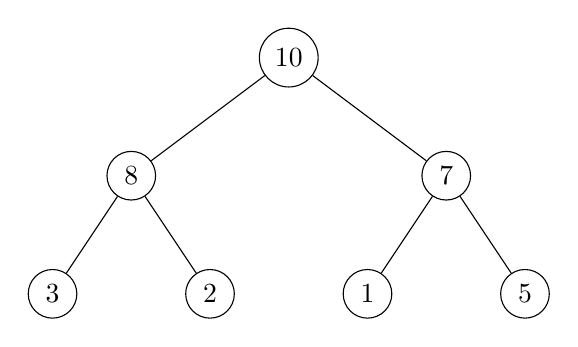
\begin{tikzpicture}[every node/.style={circle,draw},
				level 1/.style={sibling distance=40mm},
				level 2/.style={sibling distance=20mm}]
\node {10}
child { node {8} 
	child { node {3}}
	child { node {2}}
}
child { node {7} 
	child { node {1}}
	child { node {5}}
};
\end{tikzpicture}
\caption{Max heap die bewandelt wordt in ‘level order’}
\label{fig:levelorderheap}
\end{figure}
\end{opl}
\end{oef}


\begin{oef}
\papier \emph{(Examen augustus 2018)} Op de luchthaven wachten vliegtuigen op de toestemming om te landen. De vliegtuigen mogen landen in een volgorde die gebaseerd is op volgende regel: \emph{het vliegtuig met kleinste resterende hoeveelheid brandstof mag eerst landen}. De informatie met betrekking tot de brandstofhoeveelheden wordt bijgehouden in een binaire heap.

\begin{itemize}	
\item Welke is de meest aangewezen structuur: binaire min-heap of binaire max-heap?
Verklaar.




\item Volgende brandstofinhouden van vliegtuigen worden vervolgens aan de heap toegevoegd:
1225, 340, 780, 840, 996, 125, 355. Welke is de resulterende array-voorstelling van de heap?


\item Geef de resulterende array nadat 3 vliegtuigen geland zijn.

\end{itemize}	
\begin{opl}
\begin{itemize}
\item een binaire min-heap: vliegtuig met minste brandstof moet eerst van de hoop gehaald kunnen worden
\item \verb/[125,840,340,1225,996,780,355]/

\begin{figure}[htbp]
    \centering
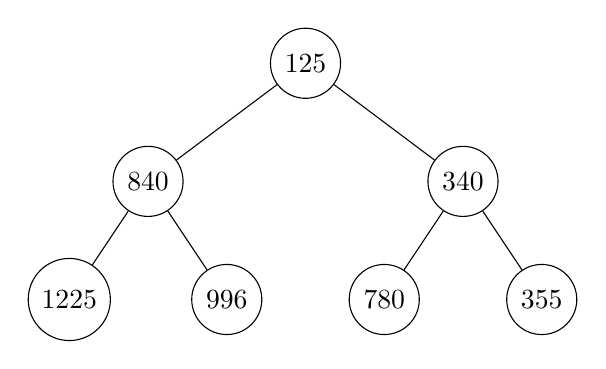
\begin{tikzpicture}[every node/.style={circle,draw},
				level 1/.style={sibling distance=40mm},
				level 2/.style={sibling distance=20mm}]
\node {125}
child { node {840} 
	child { node {1225}}
	child { node {996}}
}
child { node {340} 
	child { node {780}}
	child { node {355}}
};
\end{tikzpicture}
\caption{Min-heap van vliegtuigen}
\end{figure}
\item \verb/[780, 840, 996, 1225]/
\end{itemize}
\end{opl}
\end{oef}


\begin{oef}
\papier \emph{(Examen juni 2018)} Gegeven volgende max-heap uit figuur~\ref{fig:maxheapa} op pagina~\pageref{fig:maxheapa}. Op diepte 1 staat als root de knoop met waarde 9999. De volgende knoop heeft dan telkens als waarde één minder dan de vorige. Het laatste getal is 1. 
\begin{figure}[htbp]
    \centering
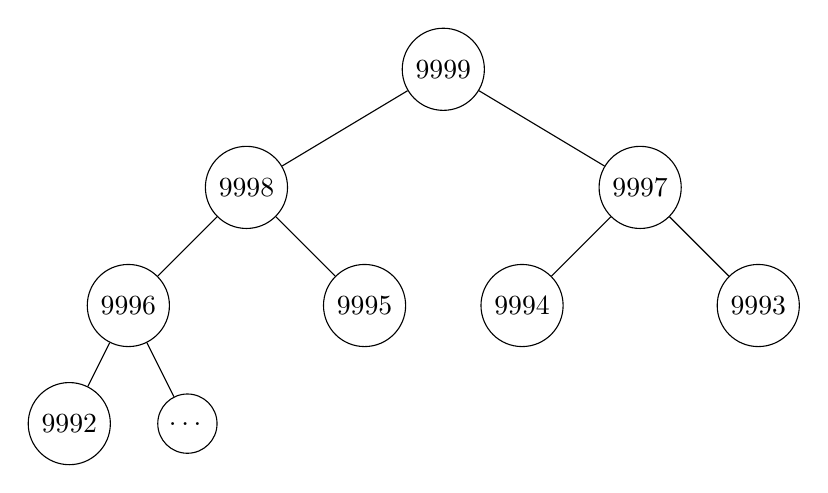
\begin{tikzpicture}[every node/.style={circle,draw},
				level 1/.style={sibling distance=50mm},
				level 2/.style={sibling distance=30mm},
				level 3/.style={sibling distance=15mm}]
\node {9999}
child { node {9998} 
	child { node {9996} 
		child { node {9992} } 
		child { node {…}}}
	child { node {9995} }
}
child { node {9997}
	child { node {9994}}
	child { node {9993}}
	};
\end{tikzpicture}
\caption{max-heap}
    \label{fig:maxheapa}
\end{figure}

\begin{enumerate}
\item Op welke diepte (= niveau) staat de knoop met waarde 1?

\item We stellen deze binaire max-heap voor met een array, dus \verb+A = [9999,9998, …, 1]+. Welke eigenschap van een binaire max-heap zorgt ervoor dat de keuze voor een array een efficiënt idee is?

\item Wat is de index van het getal 1000 in de array (+ uitleg)?

\item Wat is de waarde van het ouderelement van de knoop met waarde 1000 (+ uitleg)?

\item Geef de waarde van de twee kinderen van het element met waarde 1000 (+ uitleg).
\end{enumerate}

\begin{opl}
\begin{enumerate}
\item Op diepte 1 staat er 1 element, op diepte 2 zijn er 2, op diepte 3 zijn er 4. Op diepte 4 staan er 8. Dat zijn dus allemaal machten van 2. Reken na dat er op diepte $i$ juist $2^{i-1}$ getallen kunnen staan. Laten we nu even het \emph{cumulatieve aantal} getallen bekijken, d.w.z. het aantal getallen op een diepte gelijk aan het gegeven getal of een hoger niveau (met lagere diepte). Als voorbeeld: op diepte 4 en alle dieptes erboven (3 2, 1) staan er in totaal 15 elementen. Kijk zelf na dat het hier telkens gaat over 1 minder dan een macht van 2. Het aantal mogelijke getallen op een diepte i of hoger is dus gelijk aan $2^i - 1$. Als $i=9$ als voorbeeld kan je berekenen dat op dit niveau en alle niveau's erboven samen $2^9 - 1 = 511$ getallen kunnen staan. Van 9999 naar 1 zijn in totaal 10000 getallen. Als $i=13$ komen we aan een cumulatief aantal getallen van $2^{13}-1=8191$, wat kleiner is dan 10000. Het getal 1 staat dus op diepte 14.

\item Het feit dat een binaire max-heap compleet is: er zijn dus geen “lege plaatsen” in de array

\item Op index 0 staat het getal 9999, op index 1 het getal 9998 enz. Je merkt dat de som van de index en het getal zelf altijd 9999 is. Dat wil dus zeggen dat het getal 1000 in de array op index $9999-1000=8999$ staat.

\item Het ouderelement van het element 1000 dat op index 8999 staat is $\frac{8999-1}{2}$ afgerond naar beneden, dus index 4499. De waarde van het element op deze index van de array is dus $9999-4499=5500$.

\item De twee kinderen van het element met waarde 1000 (op index 8999) zijn de getallen op indices $8999\cdot 2 + 1$ en $8999\cdot 2 + 2$. Vermits de array maar tot index 9999 gaat, heeft de knoop met waarde 1000 geen kinderen in dit schema.
\end{enumerate}
\end{opl}
\end{oef}





\begin{oef}
\label{oef:getallen}
\papier \emph{(Examen augustus 2017)} Enkele vragen over heaps:
\begin{enumerate}
\item Een binaire min heap bestaat uit 355 getallen. Geef de indices van alle voorouders (ouder, grootouder, …) van de knoop met index 250. 

\item Een binaire min heap bestaat uit 360 getallen. Geef de indices van alle nakomelingen (kinderen, kleinkinderen, …) van de knoop met index 44. 

\item Gegeven de array-voorstelling van een binaire boom: \\ \verb+{4, 8, 10, 13, 12, 14, 12, 20, 18, 14, 17, 11}+.\\ Is deze boom een min heap? Verklaar.

\item Gegeven de array-voorstelling van een binaire boom: \\ \verb+{4, 8, 10, 13, 12, 14, 12, 20, 18, 14, 17, 11}+.  \\
Geef de array-voorstelling van de boom met als root het linkerkind van de root van deze  boom. Is deze boom een min heap?
\end{enumerate}
\begin{opl}
\begin{enumerate}
\item \verb/0,2,6,14,30,61,124/
\item \verb/89,90,179,180,181,182,359/ (de 360ste knoop heeft index 359)
\item neen, want de laatste knoop is kleiner dan zijn ouder  (zie figuur \ref{fig:geenMinHeap} op pg~\pageref{fig:geenMinHeap}) 
\begin{figure}[htbp]
    \centering
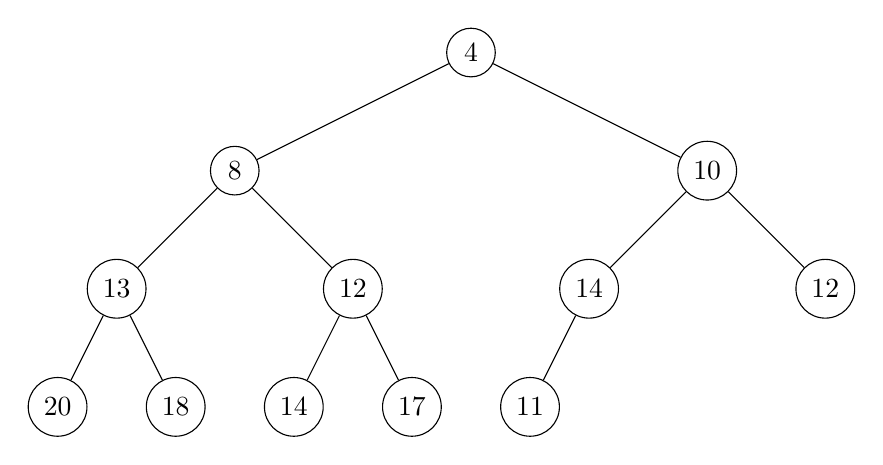
\begin{tikzpicture}[every node/.style={circle,draw},
				level 1/.style={sibling distance=60mm},
				level 2/.style={sibling distance=30mm},
				level 3/.style={sibling distance=15mm}]
\node {4}
child { node {8} 
	child { node {13} 
		child { node {20} } 
		child { node {18}}}
	child { node {12} 
		child { node {14} } 
		child { node {17}}}
}
child { node {10} 
	child { node {14} 
		child { node {11} } 
		child[missing]}
	child { node {12}}
};
\end{tikzpicture}
\caption{Oplossing bij oefening 2 van \ref{oef:getallen} - geen min-heap}
\label{fig:geenMinHeap}
\end{figure}
\item \verb/[8,13,12,20,18,14,17]/: is wel een min-heap (zie figuur \ref{fig:welMinHeap})
\begin{figure}[htbp]
    \centering
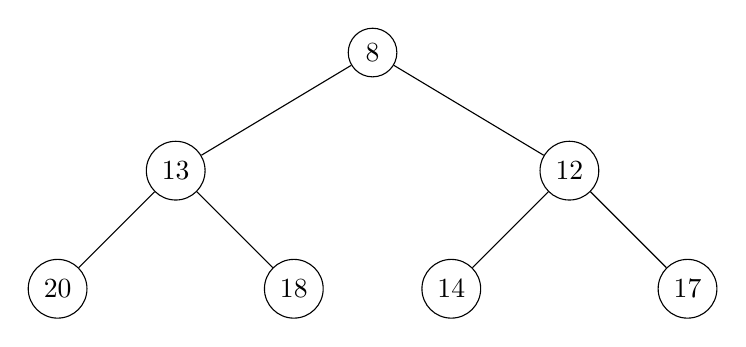
\begin{tikzpicture}[every node/.style={circle,draw},
				level 1/.style={sibling distance=50mm},
				level 2/.style={sibling distance=30mm},
				level 3/.style={sibling distance=15mm}]
\node {8} 
	child { node {13} 
		child { node {20} } 
		child { node {18}}}
	child { node {12} 
		child { node {14} } 
		child { node {17}}};
\end{tikzpicture}
\caption{Oplossing bij oefening 3 van \ref{oef:getallen} - wel min-heap}
\label{fig:welMinHeap}
\end{figure}
\end{enumerate}
\end{opl}
\end{oef}
